%!tex program = lualatex
\documentclass[answers]{exam}
\usepackage{ctex}
\usepackage{graphicx}
\usepackage[margin=2cm]{geometry}
\usepackage{amsmath, amssymb}
\usepackage{csquotes}
\usepackage{tikz, pgfplots}
\usetikzlibrary{
	angles,
	backgrounds,
	calc,
	decorations.pathmorphing,
	decorations.pathreplacing,
	decorations.text,
	intersections,
	patterns,
	quotes,
	shapes,
	shapes.symbols,
}
\pagestyle{empty}
\newcounter{xcord}
\newcounter{ycord}
\newcounter{total}
\renewcommand{\labelenumi}{\textbf{\ifnum\value{enumi}<10 0\fi\arabic{enumi})}}

\pgfplotsset{compat=1.18}

\CorrectChoiceEmphasis{\color{blue!70!green}\bfseries}
\renewcommand{\solutiontitle}{\textbf{解:}}

\usepackage{array, tabularx}
\newcolumntype{C}{>{\centering\arraybackslash}X}
\newcolumntype{B}{>{\centering\bfseries\arraybackslash}X}
\catcode`\幺=0

\begin{document}
\begin{center}
	\textbf{\large{1977 年普通高等学校招生考试(北京卷) }}

	\textbf{\LARGE{理科数学}}
\end{center}
\begin{questions}
	\question 解方程: \( \sqrt{x - 1} = 3 - x \).
	\begin{solution}
		\begin{align*}
			\sqrt{x - 1}  & = 3 - x        \\
			x - 1         & = 9 - 6x + x^2 \\
			x^2 - 7x + 10 & = 0            \\
			(x-2)(x-5)    & = 0            \\
			x_1 = 2, x_2 = 5
		\end{align*}
	\end{solution}

	\question 计算: \( 2^{-\frac12} + \frac{2^0}{\sqrt{2}} + \frac{1}{\sqrt{2} - 1}. \)

	\begin{solution}
		\begin{align*}
			\text{原式} & = \frac{1}{\sqrt{2}} + \frac{1}{\sqrt{2}} + \sqrt{2} + 1 \\
			          & = \frac{2}{\sqrt{2}} + \sqrt{2} + 1                      \\
			          & = 2\sqrt{2} + 1
		\end{align*}
	\end{solution}

	\question 已知 \( \lg2 = 0.3010, \lg3 = 0.4771, \) 求 \( \lg\sqrt{45} \).

	\begin{solution}
		\begin{align*}
			\lg\sqrt{45} & = \frac12\lg{45}                        \\
			             & = \frac12(\lg5 + \lg9)                  \\
			             & = \frac12(\lg5 + 2\lg3)                 \\
			             & = \frac12(\lg\frac{10}{2} + 2\lg3)      \\
			             & = \frac12(\lg10 - \lg2 + 2\lg3)         \\
			             & = \frac12(1 - 0.3010 + 2 \times 0.4771) \\
			             & = 0.8266
		\end{align*}
	\end{solution}

	\question 证明: \( (1 + \tan\alpha)^2 = \dfrac{1 + \sin2\alpha}{\cos^2\alpha} \)。
	\begin{solution}
		\begin{align*}
			(1+\tan\alpha)^2
			           & = \left(1 + \frac{\sin\alpha}{\cos\alpha}\right)^2  \text{(将 \(\tan\alpha = \frac{\sin\alpha}{\cos\alpha}\) 代入)} \\
			           & = \left(\frac{\cos\alpha + \sin\alpha}{\cos\alpha}\right)^2 \text{(通分并化简分母)}                                     \\
			           & = \frac{(\cos\alpha + \sin\alpha)^2}{\cos^2\alpha}                                                               \\
			           & = \frac{\cos^2\alpha + 2\cos\alpha\sin\alpha + \sin^2\alpha}{\cos^2\alpha}                                       \\
			           & = \frac{1 + 2\cos\alpha\sin\alpha}{\cos^2\alpha}                                                                 \\
			           & \text{(根据三角恒等式 \(\cos^2\alpha + \sin^2\alpha = 1\) 化简)}                                                          \\
			           & = \frac{1 + \sin2\alpha}{\cos^2\alpha}                                                                           \\
			           & \text{(利用 \(\sin2\alpha = 2\cos\alpha\sin\alpha\))}                                                              \\
			\therefore & \, (1+\tan\alpha)^2 = \frac{1 + \sin2\alpha}{\cos^2\alpha}。
		\end{align*}
	\end{solution}

	\question 求过两直线 \( x + y - 7 = 0 \) 和 \( 3x - y - 1 = 0 \) 的交点且过 \( (1, 1) \) 点的直线方程。
	\begin{solution}
		\begin{align*}
			 & \begin{cases}
				   x + y - 7 = 0, \\
				   3x - y - 1 = 0
			   \end{cases}                                                                \\
			 & \text{解得:} x = 2, \, y = 5,\text{即交点为 } (2, 5)。                               \\
			 & \text{过点 } (2,5) \text{ 和 } (1,1) \text{ 的直线斜率:} k = \frac{5 - 1}{2 - 1} = 4。 \\
			 & \text{设直线方程为:} y = 4x + a,\text{将 } (1,1) \text{ 代入,得:}                       \\
			 & a = -3。                                                                       \\
			 & \text{因此,所求直线方程为:} y = 4x - 3。
		\end{align*}
	\end{solution}

	\question 某工厂今年七月份的产值为 \( 100 \)万元,以后每月产值比上月增加 \( 20\%
	\),问今年七月份到十月份总产值是多少?

	\begin{solution}
		\begin{align*}
			\text{根据等比数列求和公式} S_n = a_1\frac{1- q^n}{1-q}                    \\
			\text{代入}  a_1 = 100, q = 1.2, n = 4  \text{得:}                  \\
			S_4 & = 100 \times \frac{1 - 1.2^4}{1 - 1.2}                     \\
			    & = 100 \times \frac{(1 - 1.2)(1 + 1.2)(1 + 1.2^2)}{1 - 1.2} \\
			    & = 100 \times 2.2 \times 2.44                               \\
			    & = 536.8 \text{(万元)}
		\end{align*}

	\end{solution}

	\question 已知二次函数 \( y = x^2 - 6x + 5 \)
	\begin{enumerate}[label=(\arabic*)]
		\item 求出它的图像的顶点坐标和对称轴方程;
		\item 画出它的图像;
		\item 分别求出它的图像和 \( x \)轴、$ y $的交点坐标.
	\end{enumerate}

	\begin{solution}
		\begin{enumerate}[label=(\arabic*)]
			\item
			      \begin{align*}
				      \text{对称轴的方程为} x = -\frac{b}{2a} & = 3,  \\
				      \text{将} x = 3 \text{代入得:} y     & = -4, \\
			      \end{align*}
			\item
			      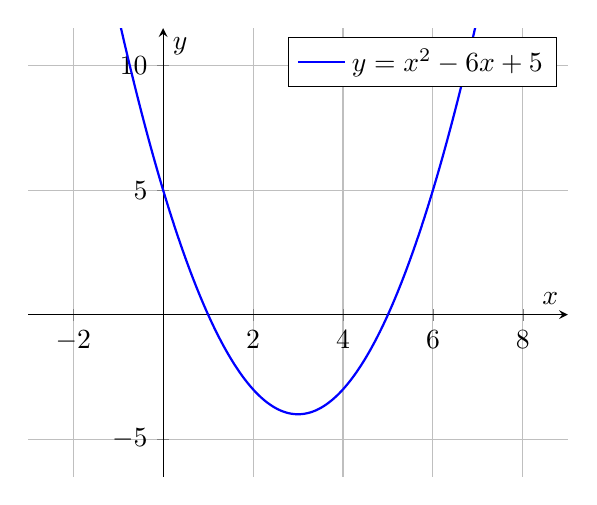
\begin{tikzpicture}
				      \begin{axis}[
						      axis lines=middle,          % 坐标轴通过原点
						      xlabel={$x$}, ylabel={$y$}, % 坐标轴标签
						      grid=major,                 % 显示网格
						      xmin=-2, xmax=8,            % x轴范围
						      ymin=-5, ymax=10,           % y轴范围
						      domain=-4:8,                % 定义函数绘制范围
						      samples=100,                % 样本点数,越大曲线越平滑
						      enlargelimits=true,         % 扩展范围
					      ]
					      % 绘制抛物线 y = ax^2 + bx + c
					      \addplot[smooth, thick, blue] {x^2 - 6*x + 5};
					      % 添加图例
					      \addlegendentry{$y = x^2 - 6x + 5$}
				      \end{axis}
			      \end{tikzpicture}
			\item \begin{align*}
				      y & = x^2 - 6x + 5                            \\
				        & = (x - 1)(x - 5)                          \\
				        & \text{则有两个交点分别为:} (1, 0) \text{和} (5, 0).
			      \end{align*}
		\end{enumerate}

	\end{solution}

\end{questions}

\end{document}
